\documentclass[a4paper, 12pt]{article}
\usepackage[small]{titlesec}
\usepackage[T2A]{fontenc}
\usepackage[utf8]{inputenc}
\usepackage[english,russian]{babel}
\usepackage{graphicx}
\usepackage{amsmath}
\usepackage{listings}
\newcommand\tab[1][1cm]{\hspace*{#1}}
\renewcommand{\baselinestretch}{1.5}

\date{Сентябрь 2020}
\begin{document}
	
	\begin{titlepage}
		\begin{center}
			
\includegraphics{msu_logo.jpg}
			\small
			~\\[0.1cm]
			Московский государственный университет имени М.В.Ломоносова
			~\\[0.1cm]
			Казахстанский филиал
			~\\[0.1cm]
			Факультет вычислительной математики и кибернетики
			~\\[1.0cm]
			\normalsize
		\end{center}
		\vspace{0.5cm}
		\begin{center}
			\textbf{\large{Отчёт по практикуму по специализации}}
			\\[1cm]
			\textbf{\large {Численное решение задачи Дирихле для уравнения
					Пуассона}}
			\\[2cm]
			\begin{normalsize}
				\vspace{2cm}
				\begin{flushright}
					\textbf{Составил}: студент Калдаров Б.М.
					\\[1cm]
					\textbf{Проверил}: преподаватель Нетесов В.В.
				\end{flushright}
				\normalsize
			\end{normalsize}
			\vfill 
			
			\small{Нур-Султан, 2020}
		\end{center} 
	\end{titlepage}
	\setcounter{page}{2}
	\tableofcontents
	
	\newpage
	\section{Постановка задачи}
	Рассматривается задача Дирихле для эллиптического уравнения
	\begin{equation}
		-Lu = f(x, y), \;\;\; (x, y) \in G,
	\end{equation}
	\begin{equation}
		u = \mu(x, y), \;\;\; (x, y) \in H.
	\end{equation}
	Пусть $\overline{G} = G + H = {0 \le x \le l_x, 0 \le y \le l_y}$ - прямоугольник, а
	\begin{equation}
		Lu = \frac{\partial}{\partial x} \bigg( p(x, y) \frac{\partial u}{\partial x} \bigg) + \frac{\partial}{\partial y} \bigg( q(x, y) \frac{\partial u}{\partial y} \bigg)
	\end{equation}

	
	Здесь $p(x, y), q(x, y)$ - достаточно гладкие функции такие, что $0 < c_1 \le p(x, y) \le c_2, 0 < d_1 \le q(x, y) \le d_2$, где $c_1, c_2, d_1, d_2$ - постоянные.
	Обозначим $A = max(c_2, d_2)$.
	Разобьём отрезок $[0, l_x]$ на $N_x$ равных частей. Обозначим $h_x = \frac{l_x}{N_x}, x_i = i h_x, 0 \le i \le N_x.$
	\newline
	Разобьём отрезок $[0, l_y]$ на $N_y$ равных частей. Обозначим $h_y = \frac{l_y}{N_y}, y_j = j h_y, 0 \le j \le N_y.$
	\newline
	
	\section{Двухслойная схема с весами}
	Построим сетку узлов:
	\begin{equation*}
		\overline{\omega_{h_x h_y}} = {(x_i, y_j), \;\;\; 0 \le i \le N_x, 0 \le j \le N_y}.
	\end{equation*}
	\newline
	Узлы $(x_i, y_j), 1 \le i \le N_x-1, 1 \le j \le N_y-1$ - внутренние, остальные, лежащие на границе прямоугольника, - граничные.
	\newline
	Пусть
	\begin{equation}
		L_1u = \frac{\partial}{\partial x} \bigg( p(x, y) \frac{\partial u}{\partial x} \bigg), \;\;\; L_2u = \frac{\partial}{\partial y} \bigg( q(x, y) \frac{\partial u}{\partial y} \bigg),
	\end{equation}
	так что
	\begin{equation}
		Lu = L_1u + L_2u.
	\end{equation}
	
	Операторы $L_1$ и $L_2$ заменим разностными операторами $\Lambda_1$ и $\Lambda_2$
	\begin{eqnarray}
		\Lambda_1 = p_{i+\frac{1}{2} j} \frac{u_{i+1 j} - u_{i j}}{h^2_x} - p_{i-\frac{1}{2} j} \frac{u_{i j} - u_{i-1 j}}{h^2_x}, \\
		\Lambda_2 = q_{i j+\frac{1}{2}} \frac{u_{i j+1} - u_{i j}}{h^2_y} - q_{i j-\frac{1}{2}} \frac{u_{i j} - u_{i j-1}}{h^2_y}.
	\end{eqnarray}
	
	Здесь
	$$ p_{i+\frac{1}{2} j} = p(x_i + \frac{h_x}{2}, y_j), \;\;\; p_{i-\frac{1}{2} j} = p(x_i - \frac{h_x}{2}, y_j), $$
	$$ q_{i j+\frac{1}{2}} = p(x_i , y_j+ \frac{h_y}{2}), \;\;\; p_{i j-\frac{1}{2}} = p(x_i , y_j- \frac{h_y}{2}).$$
	
	Обозначим
	$$ \Lambda u_{i j} = \Lambda_1 u_{i j} + \Lambda_2 u_{i j}, \;\;\; 1 \le i \le N_x-1, \;\;\; 1 \le j \le N_y-1.$$
	
	Если $u(x, y)$ имеет не менее четырех непрерывных ограниченных в рассматриваемой области $G$ производных по $x$ и по $y$, а $p(x, y)$ и $q(x, y)$ - не менее трех, то разностный оператор $\Lambda$ аппроксимирует дифференциальный $L$ со вторым порядком, т. е.
	$$ Lu - \Lambda u = O(|h|^2), |h|^2 = h^2_x + h^2_y. $$
	
	Итак, решение задачи $(1)-(2)$ свелось к решению разностной задачи Дирихле
	$$ -(\Lambda_1 u_{i j} + \Lambda_2 u_{i j}) = f_{i j}, \;\;\; 1 \le i \le N_x-1, \;\;\; 1 \le j \le N_y-1.$$
	
	Аппроксимируем задачу
	\begin{equation}
		\begin{cases}
			\frac{\partial u}{\partial t} = L_1u + L_2u + f(x, y), \\
			u|_H = \mu(x, y), \;\;\; u(x, y, 0) = u_0(x, y).
		\end{cases}
	\end{equation}
	разностной схемой
	\begin{equation}
		\frac{u^{k+1}_{i j} - u^{k}_{i j}}{\tau} = \Lambda (\sigma u^{k+1}_{i j} + (1 - \sigma)u^{k}_{i j} + f(x_i, y_j)),
	\end{equation}
	$$i = \overline{1, N_x-1}, \;\;\; j = \overline{1, N_y-1}, \;\;\; k = 0, 1, 2, ...$$
	\begin{equation}
		\begin{cases}
			u^{k+1}_{i 0} = \mu(x_i, 0), \;\;\; 1 \le i \le N_x-1, \\
			u^{k+1}_{i N_y} = \mu(x_i, l_y), \;\;\; 1 \le i \le N_x-1, \\
			u^{k+1}_{0 j} = \mu(0, y_j), \;\;\; 1 \le j \le N_y-1, \\
			u^{k+1}_{N_x j} = \mu(N_x, y_j), \;\;\; 1 \le j \le N_y-1.
		\end{cases}
	\end{equation}
	
	Решение при $k = 0$ находится из начального условия в (9)
	$$ u^0_{i j} = u_0 (x_i, y_j), \;\;\;, i = \overline{1, N_x}, \;\;\; j = \overline{1, N_y} .$$
	
	В данной работе рассматривается чисто неявная схема с значением параметра $\sigma = 1$.
	\newline
	Эта схема устойчива при любых значениях $h$ и $\tau$. Для определения $u^{k+1}_{i j}$ на каждом слое получаем линейную систему
	\begin{equation}
		u^{k+1}_{i j} - \tau (\Lambda_1 u^{k+1}_{i j} + \Lambda_2 u^{k+1}_{i j}) = u^{k}_{i j} + \tau f(x_i, y_j),
	\end{equation}
	$$i = \overline{1, N_x-1}, \;\;\; j = \overline{1, N_y-1}, \;\;\; k = 0, 1, 2, ...$$
	Матрица этой системы пятидиагональная и система решается методом матричной прогонки[1].
	\newpage
	\section{Схема переменных направлений}
	Эта схема  сочетает лучшие качества явной схемы - экономичность и неявной - устойчивость. Наряду с основными значениями $u^{k}_{i j}$ $u^{k+1}_{i j}$ вводится промежуточное значение $u^{k+\frac{1}{2}}_{i j}$, которое формально можно рассматривать как значение при $t = t_{k+\frac{1}{2}} = t_k + \frac{\tau}{2}$. Решение задачи в этом случае сводится к решению двух систем с трехдиагональными матрицами:
	\begin{equation}
		\frac{u^{k+\frac{1}{2}}_{i j} - u^{k}_{i j}}{\frac{\tau}{2}} = \Lambda_1 u^{k+\frac{1}{2}}_{i j} + \Lambda_2 u^{k}_{i j} + f(x_i, y_j))
	\end{equation}
	$$1 \le i \le N_x-1, \;\;\; 1 \le j \le N_y-1.$$
	\begin{equation}
		\frac{u^{k+1}_{i j} - u^{k+\frac{1}{2}}_{i j}}{\frac{\tau}{2}} = \Lambda_1 u^{k+\frac{1}{2}}_{i j} + \Lambda_2 u^{k+1}_{i j} + f(x_i, y_j))
	\end{equation}
	$$1 \le i \le N_x-1, \;\;\; 1 \le j \le N_y-1.$$
	$$k = 0, 1, 2, ...$$
	В граничных узлах решение должно принимать заданные в (10) значения.
	\newline
	Схема (12) неявна по направлению $x$ и явна по направлению $y$, а схема (13) ясна по направлению $x$ и неявна по направлению $y$, что позволяет использовать для нахождения решения одномерные прогонки.
	\newline
	Система (12) с учётом граничных условий (10) может быть записана в следующем виде:
	\begin{equation}
		\begin{cases}
			u^{k + \frac{1}{2}}_{0 j} = \mu(0, y_j), \\
			\overline{A_{i j}} u^{k + \frac{1}{2}}_{i-1 j} - \overline{B_{i j}} u^{k + \frac{1}{2}}_{i j} + \overline{C_{i j}} u^{k + \frac{1}{2}}_{i+1 j} = \overline{G}^{k+\frac{1}{2}_{ij}}_{i j}, 1 \le i \le N_x-1, \\
			u^{k + \frac{1}{2}}_{N_x j} = \mu(l_x, y_j).
		\end{cases}
	\end{equation}
	\newpage
	Где
	\begin{equation}
		\overline{G}^{k+\frac{1}{2}}_{i j} = -u^k_{i j} - \frac{\tau}{2} (\Lambda_2 u^k_{i j} + f(x, y)),
	\end{equation}
	$$1 \le j \le N_y-1.$$
	В итоге при каждом $1 \le j \le N_y-1.$ получили линейную замкнутую систему $N_x+1$-ого порядка относительно $u^{k + \frac{1}{2}}_{0 j}, u^{k + \frac{1}{2}}_{1 j}, ... , u^{k + \frac{1}{2}}_{N_x j}.$
	Матрица системы трёхдиагональная и решается методом прогонки [2].
	\newline
	Прогонки осуществляются вдоль строк. При $j = 0, j = N_y$ решения находятся из (10):
	\begin{equation}
		\begin{cases}
			u^{k+1}_{i 0} = \mu(x_i, 0), \;\;\; 1 \le i \le N_x-1, \\
			u^{k+1}_{i N_y} = \mu(x_i, l_y), \;\;\; 1 \le i \le N_x-1.
		\end{cases}
	\end{equation}
	Система (13) с учётом граничных условий (10) может быть записана в следующем виде:
	\begin{equation}
		\begin{cases}
			u^{k + \frac{1}{2}}_{i 0} = \mu(x_i, 0), \\
			\overline{\overline{A_{i j}}} u^{k + \frac{1}{2}}_{i-1 j} - \overline{\overline{B_{i j}}} u^{k + \frac{1}{2}}_{i j} + \overline{\overline{C_{i j}}} u^{k + \frac{1}{2}}_{i+1 j} = \overline{\overline{G}}^{k+\frac{1}{2}_{ij}}_{i j}, 1 \le j \le N_y-1, \\
			u^{k + \frac{1}{2}}_{i N_y} = \mu(x_i, l_y).
		\end{cases}
	\end{equation}
	Где
	\begin{equation}
		\overline{\overline{G}}^{k+\frac{1}{2}}_{i j} = -u^k_{i j} - \frac{\tau}{2} (\Lambda_1 u^k_{i j} + f(x, y)),
	\end{equation}
	$$1 \le i \le N_x-1.$$
	В итоге при каждом $1 \le i \le N_x-1.$ получили линейную замкнутую систему $N_y+1$-ого порядка относительно $u^{k + \frac{1}{2}}_{i 0}, u^{k + \frac{1}{2}}_{i 1}, ... , u^{k + \frac{1}{2}}_{y N_y}.$
	Матрица системы трёхдиагональная и решается методом прогонки [2].
	\newline
	Прогонки осуществляются вдоль столбцов. При $i = 0, i = N_x$ решения находятся из (10):
	\begin{equation}
		\begin{cases}
			u^{k+1}_{0 j} = \mu(0, y_j), \;\;\; 1 \le j \le N_y, \\
			u^{k+1}_{N_x j} = \mu(N_x, y_j), \;\;\; 1 \le j \le N_y.
		\end{cases}
	\end{equation}
	В нашем случае $(p(x, y) \equiv 1, q(x, y) \equiv 1, h_x = h_y = h, N_x = N_y = N)$
	\begin{equation}
		\overline{A_{i j}} = \overline{\overline{A_{i j}}} = \frac{\tau}{2 h^2}, \overline{B_{i j}} = \overline{\overline{B_{i j}}} = \frac{\tau}{h^2} + 1, \overline{C_{i j}} = \overline{\overline{C_{i j}}} = \frac{\tau}{2 h^2}.	
	\end{equation}
	
	Итак, рассмотрим алгоритм метода переменных направлений.
	\begin{enumerate}
		\item Из начального условия получаем решение при $k=0$ во всех точках сетки 	$$u^0_{i j} = u_0(x_i, y_j), 0 \le i \le N_x, 0 \le j \le N_y.$$
		\item Полагая $k = 0$, решаем методом прогонки при каждом $1 \le j \le N_y-1$ систему (14).\newline Решение при $j = 0$ и $j = N_y$ находится из  (16). Тем самым, найдено решение $u^{\frac{1}{2}}_{i j}$ на промежуточном слое $\frac{1}{2}$ во всех точках сетки.
		\item Полагая $k = 0$, решаем методом прогонки при каждом $1 \le i \le N_x-1$ систему (17). \newline Решение при $i = 0$ и $i = N_x$ находится из (19). Таким образом, найдено решение $u^{1}_{i j}$ на слое $k = 1$ во всех точках сетки.
		\item Вычислив характеристики полученного решения, увеличиваем номер слоя на единицу $(k = k+1)$ и повторяем пункты 2 и 3 пока не будет выполнен критерий окончания счёта.
	\end{enumerate}

	\newpage
	\section{Основные результаты}
	В качестве пробной функции взята функция
	$$\mu(x, y) = x^2 y + y^2 x$$ 
	Комментарии: если брать фукнцию содержащую $sin, cos$ погрешность заметно большая, а график аналитического решения "по форме" совпадает. Была взята в качество пробной функции еще "декартов лист", "леминиската" для разнообразия, но в отчете они не будут присутствовать. По программам можно лишь отметить, что схема переменных направлений работает для $n=32$, и при больших $m~\mathtt{\sim1000}$ примерно 7 сек, а матричная прогонка меньше секунды для того же $n$.
	\newpage
	Схема переменных направлений
	\begin{center}
		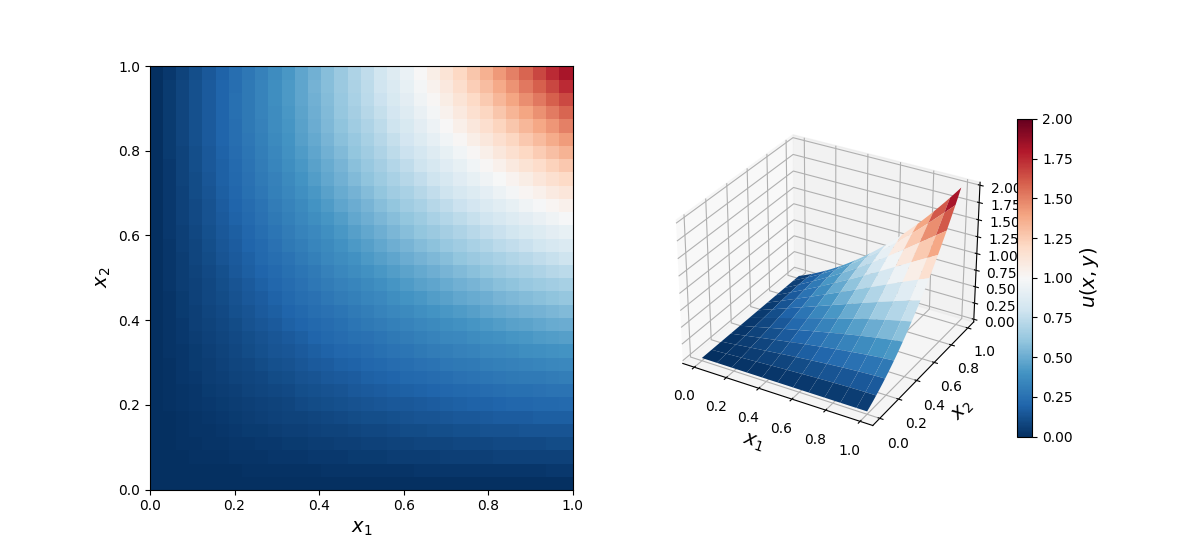
\includegraphics[scale=0.5]{plot1_1.png} \\
		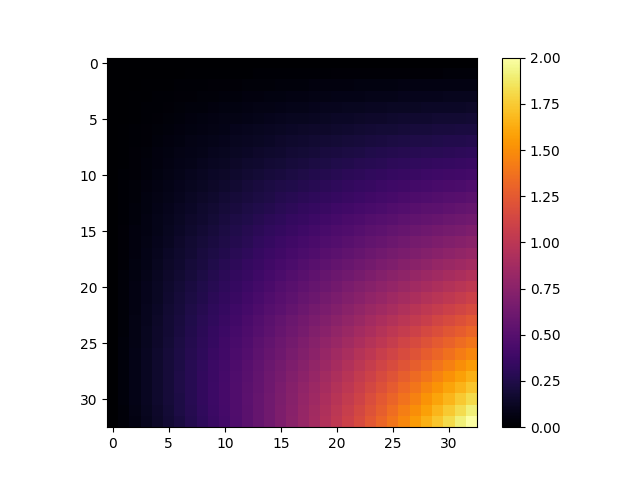
\includegraphics[scale=0.6]{plot1_2.png} \\
		\text{График для } $n = 32, ||Ua - U|| = 0.1588$.
	\end{center}

	\newpage
	Неявная схема. Метод матричной прогонки
	\begin{center}		
		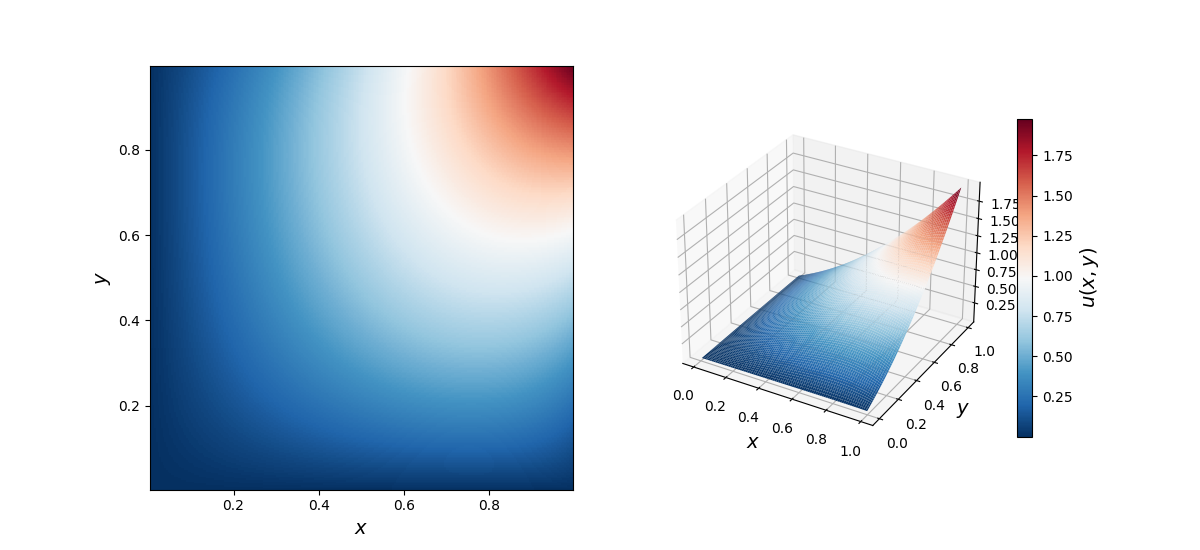
\includegraphics[scale=0.5]{plot2_1.png} \\
		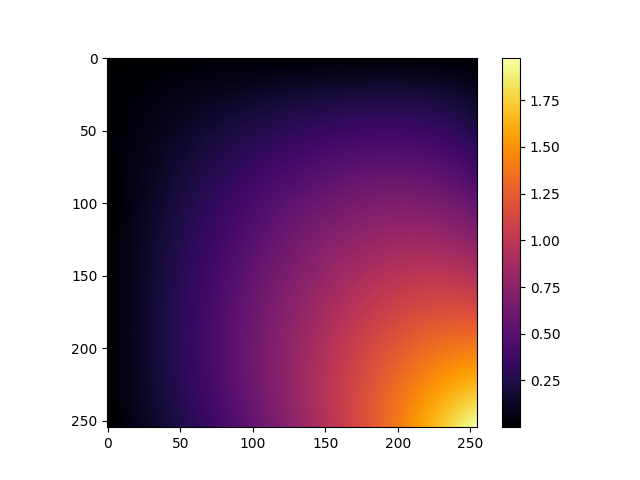
\includegraphics[scale=0.6]{plot2_2.png} \\
		\text{График для } $n = 256, ||Ua - U|| = 0.4028$.
	\end{center}
	Комментарии: при увеличении $n$ норма погрешности уменьшается. Для $n < 256$ норма чуть выше.
	
	\newpage
	\section{Листинг программы}
	\subsection{Схема переменных направлений}
	\lstset{language=Python}
	\begin{lstlisting}[
		basicstyle=\tiny, %or \small or \footnotesize etc.
		]
import numpy as np
import sys
import time as t

import matplotlib as mpl
import matplotlib.pyplot as plt
from mpl_toolkits.mplot3d.axes3d import Axes3D

def u0(x, y):
	return 0.0

def phi1(x):
	return 0.0

def phi2(x):
	return x + x*x 

def phi3(y):
	return 0.0

def phi4(y):
	return y + y*y

def ua(x, y):
	return x*x*y + y*y*x 

T = 1.0
L = 1.0
N = 32 
N1 = N+1
h = L/N
h2 = h*h
x = np.linspace(0.0, L, N1)
y = np.linspace(0.0, L, N1)

m = 1024
tau = T / m

U0 = np.zeros((N1, N1))
U_old = np.zeros((N1, N1))
U_new = np.zeros((N1, N1))

U0 = np.array([[ua(xi, yi) for yi in y] for xi in x])

U_old = U0

A = np.zeros((N1, N1))
B = np.zeros((N1, N1))
C = np.zeros((N1, N1))
D = np.zeros((N1, N1))
for i in range(N1):
for j in range(N1):
A[i, j] = -1/(2*h2)
B[i, j] = 1/tau + 1/h2
C[i, j] = -1/(2*h2)

alpha = np.zeros(N1)
beta = np.zeros(N1)

start = t.time()

for k in range(m):
	for i in range(N1):
		U_old[0, i] = phi3(y[i])
		U_new[0, i] = phi3(y[i])
		U_old[N, i] = phi4(y[i])
		U_new[N, i] = phi4(y[i])
		
	for i in range(1, N):
		for j in range(1, N):
			D[i, j] = U_old[i, j]/tau + (U_old[i, j-1] - 2*U_old[i, j] + U_old[i, j+1]) / (2*h2)
		
		for j in range(1, N):
			alpha[1] = 0
			beta[1] = phi3(x[j])
			for i in range(1, N):
			alpha[i+1] = -C[i, j] / (B[i, j] + A[i, j] * alpha[i])
			beta[i+1] = (D[i, j] - A[i, j]*beta[i])/(B[i, j] + A[i, j]*alpha[i])
			U_old[N, j] = phi4(x[j])
			for i in range(N-1, 0, -1):
				U_old[i, j] = alpha[i+1] * U_old[i+1, j] + beta[i+1]
	
	for i in range(N1):
		U_old[0, i] = phi1(x[i])
		U_new[0, i] = phi1(x[i])
		U_old[N, i] = phi2(x[i])
		U_new[N, i] = phi2(x[i])
		
	
	for i in range(1, N):
		for j in range(1, N):
			D[i, j] = U_old[i, j]/tau + (U_old[i, j+1] - 2*U_old[i, j] + U_old[i, j-1]) / (2*h2)
		
		for i in range(1, N):
			alpha[1] = 0
			beta[1] = 0 
			for j in range(1, N):
			alpha[j+1] = -C[i, j] / (B[i, j] + A[i, j] * alpha[i])
			beta[j+1] = (D[i, j] - A[i, j]*beta[j])/(B[i, j] + A[i, j]*alpha[j])
			U_new[i, N] = phi2(y[i])
			for j in range(N-1, 0, -1):
				U_new[i, j] = alpha[j+1] * U_new[i, j+1] + beta[j+1]
		
	U_old[:, :] = U_new[:, :]

end = t.time()
print('time = ', end-start, sep='')

Ua = np.array([[ua(xi, yi) for yi in y] for xi in x])

av_err = np.max(np.abs(Ua-U_new))
print(f"|Ua-U| = {av_err}")

mx = U_new.max()
mn = U_new.min()
X, Y = np.meshgrid(x, x)
fig = plt.figure(figsize=(12,5.5))
cmap = mpl.cm.get_cmap('RdBu_r')
ax =  fig.add_subplot(1,2,1)
c = ax.pcolor(X, Y, U_new, vmin=mn, vmax=mx, cmap=cmap)
ax.set_xlabel(r"$x_1$", fontsize=14)
ax.set_ylabel(r"$x_2$", fontsize=14)

ax =  fig.add_subplot(1,2,2, projection='3d')
p = ax.plot_surface(X, Y, U_new, vmin=mn, vmax=mx, rstride=3, cstride=3, linewidth=0, cmap=cmap)
ax.set_xlabel(r"$x_1$", fontsize=14)
ax.set_ylabel(r"$x_2$", fontsize=14)

cb = plt.colorbar(p, ax=ax, shrink=0.75)
cb.set_label(r"$u(x, y)$", fontsize=14)

fig1, ax1 = plt.subplots()
cs = plt.imshow(U_new, cmap='inferno')
fig1.colorbar(cs)
plt.show()
	\end{lstlisting}
	\subsection{Метод матричной прогонки}
	\lstset{language=Python}
	\begin{lstlisting}[
		basicstyle=\tiny, %or \small or \footnotesize etc.
		]
import numpy as np
import math
import sys
import scipy.linalg as sl
import time as t
import matplotlib.pyplot as plt
import matplotlib as mpl
from mpl_toolkits.mplot3d.axes3d import Axes3D


def f(x, y):
	return 5*x + 2*x*y

def left(y):
	return 0.0

def right(y):
	return y+y*y

def bottom(x):
	return 0.0

def top(x):
	return x*x+x

def ua(x, y):
	return x*x*y + y*y*x


def sweep(m, C, F):
	Alfa = [np.zeros((m,m))] * m
	beta = np.zeros((m, m))
	
	Alfa[0] = sl.inv(D)
	beta[0] = np.dot(Alfa[0], F[0])
	
	for i in range(m-1):
		tmp = sl.inv(D-Alfa[i])
		Alfa[i+1] = tmp
		beta[i+1] = np.dot(tmp, F[i+1] + beta[i])
	
	X = beta
	
	for i in range(m-2, -1, -1):
		X[i] = np.dot(Alfa[i], X[i+1]) + beta[i]
	
	return X

if len(sys.argv) < 2:
	print("N missing")
	exit(1)

n = int(sys.argv[1])
nm1 = n-1
nm2 = n-2
np1 = n+1

h = 1.0/n
h2 = h*h

x = np.linspace(0.0, 1.0, np1)
y = np.linspace(0.0, 1.0, np1)

F = np.zeros((nm1, nm1))
for i in range(nm1):
	F[0, i] += left(y[i+1]) / h2
	F[nm2, i] += right(y[i+1]) / h2
	F[i, 0] += bottom(x[i+1]) / h2
	F[i, nm2] += top(x[i+1]) / h2

	for j in range(nm2):
		F[i, j] += f(x[i+1], y[i+1])

F *= h2

D = np.ones((nm1, nm1))
D = 5 * np.eye(nm1) - sl.triu(sl.tril(D, 1), -1)

start = t.time()
U = sweep(nm1, D, F).transpose()
end = t.time()
print('time = ', end-start, sep='')

Ua = np.zeros((np1, np1))
for i in range(np1):
for j in range(np1):
Ua[i, j] = ua(x[i], y[j])

#ans = np.max(np.abs(Ua-U))

#print(f"|Ua-U| = {ans}")

x_i = x[1:n]
y_i = y[1:n]

mx = U.max()
mn = U.min()
print(mx, mn)
X, Y = np.meshgrid(x_i, x_i)

fig = plt.figure(figsize=(12, 5.5))
cmap = mpl.cm.get_cmap('RdBu_r')
ax = fig.add_subplot(1,2,1)
c = ax.pcolor(X, Y, U, vmin=mn, vmax=mx, cmap=cmap)
ax.set_xlabel(r"$x$", fontsize=14)
ax.set_ylabel(r"$y$", fontsize=14)

ax = fig.add_subplot(1, 2, 2, projection='3d')
p = ax.plot_surface(X, Y, U, vmin=mn, vmax=mx, rstride=3, cstride=3, linewidth=0, cmap=cmap)
ax.set_xlabel(r"$x$", fontsize=14)
ax.set_ylabel(r"$y$", fontsize=14)

cb = plt.colorbar(p, ax=ax, shrink=0.75)
cb.set_label(r"$u(x, y)$", fontsize=14)

fig1, ax1 = plt.subplots()

cs = plt.imshow(U, cmap='inferno')
fig1.colorbar(cs)
plt.show()
	\end{lstlisting}
	\newpage
	\section{Список литературы}
	
	\begin{enumerate}
		\item \textbf{Пакулина А.Н.} Практикум по методам вычислений. Часть 2. СПб., СПбГУ, 2019. – 113 с.
		\item \textbf{Самарский А.А, Гулин А.В.} Численные методы математической физики. Наука, 2000. - 310 с.
	\end{enumerate}
	
	
	
\end{document}
